\chapter{Etat de l'art}
\label{chap:stateoftheart}

Ce projet ne part pas de zéro.
En effet, Mme Yerly est une enseignante de mathématiques à la \acrshort{heia-fr} qui a proposé un modèle de \acrlong{ml} pour prédire le point d'ébullition d'un liquide ionique.
Elle a réalisé ce projet\cite{IL_SVM_report} avec l'aide de M Marti en se basant sur une étude d'un chercheur qui s'appelle Wang\cite{WANG2021432}.

Le modèle qu'ils ont réalisé obtient des résultats satisfaisants mais il est limité par les données qu'ils ont utilisées.
En effet, ce modèle se base seulement sur la présence ou non de certaines molécules dans la composition du liquide ionique.

% -----------------------------------------------------------------------------
\section{Analyse}
\label{sec:stateoftheart:analysis}
L'idée de ce projet est de déterminer le point de fusion d'un liquide ionique à partir de la présence ou non de molécules.
L'étude de bases\cite{WANG2021432} fournie des données et certaines d'entre elles ont été ajoutées par la HEIAFR.
Le but est de préprocesser ces données avec l'algorithme de normalisation \acrshort{minimax} puis de faire une régression avec \acrshort{svm}.

\subsection{Données}
Les données de base sont fournies dans un tableau excel\cite{SVM_data} mais elles se trouvent aussi dans le nouveau fichier créé pour ce projet\cite{New_data}.
Le dataset contient 102 colonnes dont deux qui sont inutiles car ce sont les noms des anions et des cations.
Les 99 features ont des valeurs entre 0 et 30 et représentent la présence ou non d'une molécule dans la composition du liquide ionique.
Le dataset d'entraînement contient 600 lignes qui sont toutes complètes et aucune ligne n'est dupliquée.
La valeur cible est la colonne \texttt{Exp (K)} qui représente le point de fusion en degrés Kelvin.
La moyenne des points de fusions est de 322,29 K et la médiane de 318,5 K.
Les valeurs se situent entre 177,15 et 550,15 Kelvin ce qui nous fait un écart-type de 54, 37 K.
Voici l'historgramme des points de fusion selon pandas-profiling\cite{pp_old}:
\begin{center}
    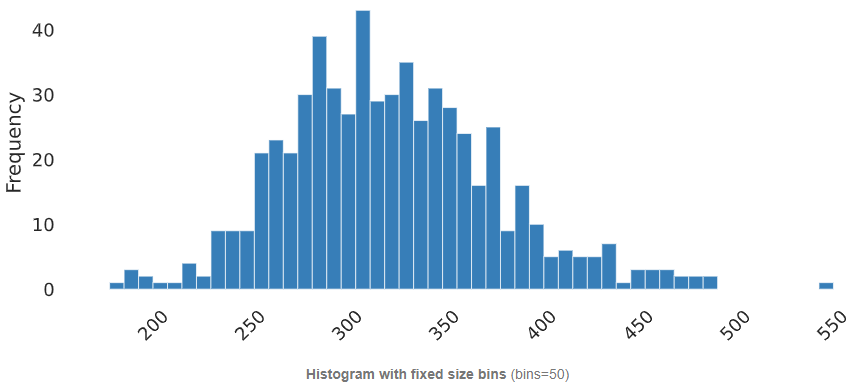
\includegraphics[width=140mm]{img/histogram_exp_old_pp.png  }
    \captionof{figure}{Histrogramme fourni par pandas profiling des points de fusions des données de base}
\end{center}

\subsection{Préprocessing}
Le preprocessing des données est important car il permet de les mettre en forme ces dernières dans un intervalle défini.
Ceci permet d'éviter un problème de poids inégale entre les features dus à la grandeur des distances.
Il existe plusieur méthodes de scalling et elles sont presque toutes utilisables avec scikit-learn\cite{scikit-learn}.
L'algorithme de normalisation utilisé dans ce cas est \acrshort{minimax} et il est plus détaillé dans le chapitre \ref{analyse:ml:normalisation:minimax}.

\subsection{Régression}
La régression consiste à adapter une fonction afin de prédire une valeur numérique.
Dans ce projet, le but est de trouver les températures de fusion des liquides ioniques à partir de la présence ou non de molécules.
La première version de ce projet utilise l'algorithme \acrfull{svm} de la libraire LibSVM\cite{libsvm_doc}.
Plus précisément, il utilise une variante appelée \acrshort{nusvr} qui est détaillée dans le chapitre \ref{analyse:ml:algorithme:svm}.
Le but est de reproduire les résultats en utilisant la librairie scikit-learn\cite{scikit-learn} qui est une librairie python qui permet de faire du \acrlong{ml}.


% -----------------------------------------------------------------------------
\section{Conception}
Lors de l'obtention des résultats de la part de Mme Yerly et M Marti, ils ont du emprunter un certain cheminement.
Le but est de reproduire fidellement ce cheminement mais avec le nouveau fichier\cite{New_data} et \acrlong{sklearn}\cite{scikit-learn}.

\subsection{Préprocessing}
Le preprocessing utilisé est l'algorithme \acrshort{minimax} qui permet de normaliser les données.
Il est appliqué sur les features et la valeur cible.
Il ne faudra donc pas oublier de dénormaliser les valeurs prédites.

\subsection{Régression}
\label{sec:conception_regression}
Mme Yerly er M Marti ont utilisé la librairie libsvm\cite{libsvm_doc} pour faire la régression.
Pour ce projet, il faut utiliser la librairie scikit-learn\cite{scikit-learn} car elle permte de changer plus facilement d'algorithme et propose d'autres fonctionalitées.
Ceci ne devrait pas poser problème car elle utilise la librairie libsvm\cite{libsvm_doc} pour faire les \acrlong{svm}.

Une fois que la reproduction est faite, il est intéressant de tester d'autres algorithmes pour voir si les résultats sont meilleurs.

\subsubsection{Les hyper paramètres}
Les hyper paramètres optimaux sont donnés dans le rapport\cite{IL_SVM_report} de Mme Yerly et M Marti ets ont les suivants: texttt{-s 4 -t 2 -g 0.0272 -c 65}.
Si on traduit ces paramètres pour scikit-learn nous obtenons le tableau suivant:
\begin{table}[ht]
    \centering
    \begin{tabular}{|l|l|}
    \hline
    \textbf{LibSVM} & \textbf{Scikit-learn} \\ \hline
    -s 4            & Algorithme \acrshort{nusvr}      \\ \hline
    -t 2            & Regression \acrshort{nusvr}    \\ \hline
    -g 0.0272       & gamma=0.0272          \\ \hline
    -c 65           & C=65                  \\ \hline
    \end{tabular}
    \caption{Traduction des hyper paramètres de libsvm vers scikit-learn}
\end{table}


% -----------------------------------------------------------------------------
\section{Implémentation}
La reproduction des résultats s'obtient assez facilement avec la libraire scikit-learn\cite{scikit-learn}.
Il faut lire les données, les modifier et entrainer le modèle avec.

Pour reproduire les résultats, il suffit d'utiliser le script\cite{fusion_perdictor} de la manière suivante:
\begin{lstlisting}[language=bash]
    python fusion_predictor.py -ob -m minmax -a nusvr train
\end{lstlisting}
Il construira le dataset avec les données de bases et entraînera le modèles de l'étude de Mme Yerly et M Marti.

Le paramèptre -o permet de lire les anciennes données.
-n et -a permettent de choisir le scaler et l'algorithme.
Le paramètre -b indique si les targets doivent normalisées.
Le dernier paramètre indique l'action que nous voulons faire.

\subsection{Lecture des données}
Les données sont stockées dans un ficher Excel qui peut être lu avec la librairie \acrfull{pandas}.
Pour lire les données il ne faut pas oublier d'enlever les lignes et les colonnes non numériques.

\subsection{Préparation des données}
Les données doivent être prépocesser avec \acrshort{minimax} de scikit-learn.
Pour avoir les mêmes résultats que Mme Yerly et M Marti, il faut normaliser les features et la target.
Comme les données cibles prédites seront entre 0 et 1, il ne faudra pas oublier des dénormaliser avant de calculer quelquonques métriques.

\subsection{Entrainement du modèle}
L'entrainement du modèle se fait simplement avec sckiti-learn et les paramètres défini dans le chapitre \ref{sec:conception_regression}.


% -----------------------------------------------------------------------------
\section{Résultats}
Mme Yerly et M Marti ont entrainé leur modèle pour avoir le meilleure résultat prossible.
Voici une comparaison des résultats obtenus avec les données d'entraînement et de test:

\begin{table}[ht]
    \centering
    \begin{tabular}{l|cc|cc|}
    \cline{2-5}
    \multicolumn{1}{c|}{}              & \multicolumn{2}{c|}{\textbf{Etude}}                            & \multicolumn{2}{c|}{\textbf{Reproduction}}                     \\
    \multicolumn{1}{c|}{\textbf{}}     & \multicolumn{1}{c|}{\textbf{Training set}} & \textbf{Test set} & \multicolumn{1}{c|}{\textbf{Training set}} & \textbf{Test set} \\ \hline
    \multicolumn{1}{|l|}{\textbf{\acrshort{mse}}} & \multicolumn{1}{c|}{386.85}                & 515.47            & \multicolumn{1}{c|}{386.97}                & 516.12            \\ \hline
    \multicolumn{1}{|l|}{\textbf{\acrshort{mae}}} & \multicolumn{1}{c|}{?}                     & ?                 & \multicolumn{1}{c|}{13.18}                 & 18.1              \\ \hline
    \multicolumn{1}{|l|}{\textbf{\acrshort{me}}}  & \multicolumn{1}{c|}{?}                     & ?                 & \multicolumn{1}{c|}{103.1}                 & 69.78             \\ \hline
    \multicolumn{1}{|l|}{\textbf{$R^2$}}   & \multicolumn{1}{c|}{87\%}                  & 82.5\%            & \multicolumn{1}{c|}{86.89\%}               & 81.79\%           \\ \hline
    \end{tabular}%
    \caption{Comparaison des résultats entre l'étude et la reproduction}
\end{table}

La légère différence n'est pas significative.
Si on affiche les données prédites et les données réelles, on obtient le graphique suivant:

\begin{figure}[ht]
    \centering
    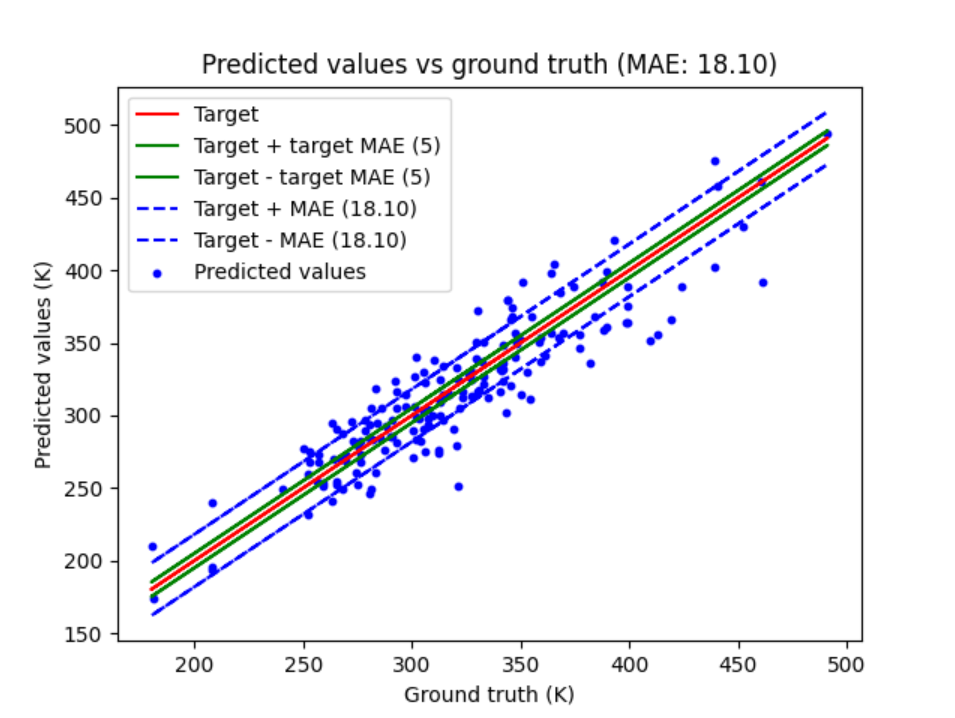
\includegraphics[width=0.8\columnwidth]{img/graphic_reproduction_result.png}
    \caption{Comparaison des données prédites et des données réelles pour la reproduction}
\end{figure}

L'objectif de l'institut est de prédire des données avec un \acrlong{mae} de cinq.
Le modèle actuel est très loin de cet objectif.

\subsection{D'autres algorithmes}
Scikit-learn permet de facilement changer d'algorithme.
Pour lancer la reproduction avec un autre algorithme, il faut modifier le paramètre -a.
Voici les résultats obtenus avec les autres algorithmes:

\begin{table}[ht]
    \centering
    \begin{tabular}{l|c|c|c|c|}
    \cline{2-5}
    \multicolumn{1}{c|}{\textbf{}}     & \textbf{nuSVR} & \textbf{SVR} & \textbf{Gradient boosting} & \textbf{Random forest} \\ \hline
    \multicolumn{1}{|l|}{\textbf{\acrshort{mse}}} & 516.12         & 870.3        & 1148.9                     & 959.36                 \\ \hline
    \multicolumn{1}{|l|}{\textbf{\acrshort{mae}}} & 18.1           & 23.91        & 26.17                      & 22.67                  \\ \hline
    \multicolumn{1}{|l|}{\textbf{\acrshort{me}}}  & 69.78          & 86           & 105.95                     & 116.45                 \\ \hline
    \multicolumn{1}{|l|}{\textbf{$R^2$}}   & 81.79\%        & 69.29\%      & 59.47\%                    & 66.15\%                \\ \hline
    \end{tabular}%
    \caption{Résultats des autres algorithmes avec les données de bases}
\end{table}

Les meilleurs résultats sont effectivement ceux obtenus par Mme Yerly et M Marti.